% Draft for the First Workshop on Medical World Models (MedWM) at AAAI-27.
% AAAI two-column format. Put the style and bibliography style from the AAAI author kit
% (https://aaai.org/authorkit27/) in this folder: aaai2027.sty/.bst, aaai27.sty/.bst, or
% the AAAI-26 kit's aaai2026.sty/.bst (used here). Without them a plain two-column preview is built.
% Single-blind workshop: the kit's [submission] option (anonymous) is not used.
% Tables and figures: python scripts/paper_tables.py and scripts/audit_v3_extra.py.
\newif\ifaaaikit
\def\aaaistyle{}
\IfFileExists{aaai2027.sty}{\aaaikittrue\def\aaaistyle{aaai2027}}{%
  \IfFileExists{aaai27.sty}{\aaaikittrue\def\aaaistyle{aaai27}}{%
  \IfFileExists{aaai2026.sty}{\aaaikittrue\def\aaaistyle{aaai2026}}{\aaaikitfalse}}}
\ifaaaikit
  \documentclass[letterpaper]{article}
  \usepackage{\aaaistyle}
  \usepackage{times}
  \usepackage{helvet}
  \usepackage{courier}
  \usepackage[hyphens]{url}
  \usepackage{graphicx}
  \urlstyle{rm}
  \def\UrlFont{\rm}
  \usepackage{natbib}
  \usepackage{caption}
  \frenchspacing
  \setlength{\pdfpagewidth}{8.5in}
  \setlength{\pdfpageheight}{11in}
\else
  \documentclass[10pt,twocolumn,letterpaper]{article}
  \usepackage[margin=0.75in]{geometry}
  \usepackage{times}
  \usepackage[hyphens]{url}
  \usepackage{graphicx}
  \usepackage[numbers]{natbib}
  \frenchspacing
\fi
\usepackage{amsmath}
\usepackage{amssymb}
\usepackage{booktabs}
\graphicspath{{../figures/}}
\setcounter{secnumdepth}{1} % numbered sections (allowed by the AAAI template), so appendix references resolve

\title{Don't Learn Pharmacology from Confounded Data:\\
Grey-Box World Models for Counterfactual Clinical Simulation}
\ifaaaikit
\author{Param Thakkar}
\else
\author{Param Thakkar\\Independent\\\texttt{paramthakkar864@gmail.com}}
\date{}
\fi
\ifaaaikit
\affiliations{Independent\\
paramthakkar864@gmail.com}
\fi

\newcommand{\Emax}{E_{\max}}
\ifaaaikit\nocopyright\fi % workshop submission: the copyright notice is for camera-ready only

\begin{document}
\maketitle

\begin{abstract}
A medical world model is useful for planning only if it answers ``what if we dosed differently?'' correctly. In clinical records sicker patients receive more drug, so a model fitted to them can learn that a drug makes patients worse. We build a benchmark on a sepsis simulator and the UVA/Padova glucose simulator in which one setting moves the training data from random dosing to dosing purely by hidden severity, and score models on the effects they predict, the doses they would choose and the danger they foresee. Under full confounding, four sequence models (GRU, GRU-ODE, CRN, Transformer) predict effects no better than assuming the drug does nothing and dose worse than a fixed dose, even as their forecasts of the recorded data improve. Our grey-box world model lets a dose act only through pharmacology with a fixed direction of effect, and sets one multiplier per drug on 100 randomised patients. It keeps its effect skill at every confounding level (0.64 on sepsis, 0.50 on glucose), with as few as 25 randomised patients and with priors wrong by up to fourfold. Fine-tuning the baselines on the same patients recovers much of what they lost, but the grey-box model stays ahead, also when planning, in two tests specified before their fresh seeds were trained (80 of 80 comparisons). Inverse-probability weighting does not help, even when it is given the true severity. To screen a model without a simulator, we test whether its errors on 72 randomised patients depend on the dose: across 312 models this flagged 108 of the 110 seriously broken ones, including 12 of 13 fine-tuned ones, but also 80 of the other 202. The grey-box model is given the form of the true pharmacology, so these results show what such knowledge buys when it is approximately right; it forecasts the recorded data worse than unadjusted baselines and misjudges some effect sizes.
\end{abstract}

\section{Introduction}

A world model \citep{ha2018world,hafner2020dream} is a simulator learned from data. In medicine the appeal is clear: try a treatment on a model of the patient before trying it on the patient. This works only if the model answers one kind of question correctly: \emph{what would happen if we gave a different dose?}

Clinical records make that question hard. Take insulin. A patient with very high glucose receives more insulin, and their glucose stays high for some time anyway. A model trained on these records sees large doses alongside high glucose, and can conclude that insulin \emph{raises} glucose. This is called confounding by indication \citep{kyriacou2016confounding}: the dose is chosen because of how sick the patient is, and part of that sickness is not recorded.

A model that makes this mistake can still look excellent. Under the clinician's usual dosing, a large dose really is a good clue that a patient is sick, so reading severity from the dose improves forecasts. The usual measure, error on the recorded data (\emph{factual error}), gets better while the model's understanding of the drug gets worse. A hospital also has no simulator to reveal the truth, so the mistake may never be noticed.

We make three contributions:
\begin{itemize}
\item \textbf{A benchmark for this failure.} Two simulators, each with one setting $\lambda$ that controls how strongly dosing follows hidden severity. Models are scored on what matters for treatment: the predicted change from a dose change, the doses they would choose, and the dangerous events they foresee. Pass marks were fixed before the final runs.
\item \textbf{A grey-box world model} built from standard parts, which tests one design rule: the dose may reach the outcome only through pharmacology. We write in what pharmacology already knows (which way a drug pushes the outcome, and the shape of its dose--response and timing), learn the patient's course without treatment with a neural network, and set the \emph{size} of each drug's effect using a small randomised set of patients.
\item \textbf{A screen that needs no simulator.} On a small randomised hold-out set, we test whether a model's errors depend on the dose. It uses only data a hospital could have, and we measure on 312 trained models whether it catches the ones that are truly broken.
\end{itemize}
We say which properties hold by construction and which are measured, and we report where our model does worse. Our claim is conditional: the grey-box model is told the form of the simulators' pharmacology (with priors we can make wrong), so the comparison measures what approximately correct pharmacological knowledge buys over learning effects from confounded data, not that the model would find unknown mechanisms.

\medskip
\noindent\fbox{\parbox{\dimexpr\columnwidth-2\fboxsep-2\fboxrule}{\small
\textbf{In short.}
\begin{itemize}
\setlength{\itemsep}{1pt}
\item Trained on confounded records, standard models can believe that insulin raises glucose, while their forecasts of the recorded data improve.
\item A model in which the dose can only act through fixed-direction pharmacology does not make this mistake. Its effects come from the pharmacology; its learned course matters for dosing only where the untreated course is complex (glucose, not sepsis).
\item 100 randomised patients rescue most standard models, and our model still does better, also when planning (confirmed on fresh seeds); it needs only 25 and keeps its effects even with the 50 mildest, whereas fine-tuning needs sick ones. Inverse weighting does not help, even given the true severity.
\item Testing whether a model's errors on randomised patients depend on the dose caught nearly every broken model without a simulator, but rarely wrong timing, and it flags many moderately wrong models.
\item What does not hold: the fluid effect is too small, a prior of the wrong form costs up to 40\% of effect skill, and all of this is on simulators.
\end{itemize}}}
\medskip

\section{Related Work}

Deep models of treatment outcomes over time include Counterfactual Recurrent Networks (CRN) \citep{bica2020crn}, which balance representations across treatments, and the Causal Transformer \citep{melnychuk2022causal}. These handle confounding by \emph{recorded} variables; our confounder is hidden. We chose this case on purpose: it is the one that adjustment for recorded variables cannot fix by design, and in intensive care much of what drives a dose (the bedside impression of how sick a patient is) is not recorded. We include CRN and inverse weighting to show that methods built for recorded confounders do not fix it, not as competitors expected to win; where the recorded outcome reveals part of the severity (glucose at low $\lambda$), weighting does help a little. A benchmark in which dosing also follows recorded variables, where these methods should do better, is future work. The Time Series Deconfounder \citep{bica2020deconfounder} infers substitutes for hidden confounders from multiple treatment assignments. \citet{soleimani2017treatment} address the same clinical question with Gaussian processes.

Hybrid models combine mechanistic and neural parts. Neural-PK/PD \citep{lu2021neuralpkpd} embeds pharmacological structure in a neural ODE; \citet{qian2021integrating} integrate expert ODEs into latent neural ODEs; APHYNITY \citep{yin2021aphynity} completes an incomplete physical model with a network kept as small as possible. Our model belongs to this family and uses the classical effect-compartment delay \citep{sheiner1979ke0}; we do not claim a new architecture. These works judge a model mainly by how well it forecasts; to our knowledge none varies how strongly dosing follows hidden severity, or scores hybrid and black-box models on the effects they predict and the doses they would choose as it does. What is new here is that comparison, the finding from it that the route of the dose matters more than having a mechanistic block, and a way to check a model without a simulator. Our question is different from forecasting accuracy: which design choices keep answers to ``what if'' questions correct under hidden confounding, and how to tell when they are not. Our ablations show that including mechanistic parts is not enough; what matters is the route by which the dose reaches the outcome. Using a small randomised set to correct estimates from confounded data follows \citet{kallus2018grounding}, who do so for static treatment effects; we do it for dynamic dose--response in a world model, and also use a randomised set to check a model. For prediction intervals we use split conformal calibration \citep{lei2018conformal}.

\section{A Confounding-Stress Benchmark}

\paragraph{How doses are chosen.} For each drug with maximum dose $a_{\max}$,
\begin{equation}
a_t = \mathrm{clip}\big(\lambda\, d(s_t) + (1-\lambda)\, r_t + \epsilon_t,\; 0,\; a_{\max}\big).
\end{equation}
Here $s_t$ is the patient's true sickness, which no model sees, $d(s_t)$ is the dose that sickness calls for, $r_t$ is a random dose held for a while, and $\epsilon_t$ is small noise. At $\lambda=0$ dosing is random, like a randomised trial. At $\lambda=1$ dosing follows sickness alone. Patients, noise, observation patterns and data splits are the same at every $\lambda$, so confounding is the only thing that changes. Each dataset has 2000 patient trajectories, split 1400/300/300.

\paragraph{Sepsis.} A small heart-and-circulation simulator we built for this study, with 15-minute steps over 48 h. It is not clinically validated. Mean arterial pressure (MAP), heart rate and lactate are observed at irregular times. The drugs are norepinephrine (NE), which raises pressure, and fluids, which fill a leaking blood volume. Low pressure makes the patient sicker. The outcome is MAP.

\paragraph{Glucose.} The UVA/Padova type 1 diabetes model \citep{man2014uvapadova}, using the equations and ten adult virtual patients of simglucose \citep{xie2018simglucose}, with 5-minute steps over 24 h. Only continuous glucose readings are observed. The drugs are basal insulin and boluses; meals are given as known inputs. Sickness is how far plasma glucose is above target.

\paragraph{What we measure.} Each model sees the start of a test trajectory (6 h on sepsis, 4 h on glucose) and then predicts forward with no further readings: 5 h on sepsis and 6 h on glucose, long enough for insulin's effect to build. For the true answer, we replay the simulator from the patient's true state with the same random noise. There are 300 test patients. Metrics concern the outcome variable unless stated.
\begin{itemize}
\item \emph{Effect skill}: how well a model predicts the change caused by altering the first drug (NE, basal insulin), by stopping it, raising it 30\%, or setting it to 80\% of maximum. With true change $\Delta$, it is $1-\mathrm{RMSE}(\widehat{\Delta}-\Delta)/\mathrm{RMS}(\Delta)$. A score of 1 is perfect, 0 is no better than saying the drug does nothing, and below 0 is worse than that.
\item \emph{CF RMSE}: normalised forecast error over all observed variables when doses are changed, under six dosing policies (random, aggressive, conservative, dose $\pm$30\%, and a one-step flip). For boluses, which are occasional, the first three keep the recorded timing.
\item \emph{CF coverage}: how often the truth falls inside the 90\% prediction interval under the three changes above. We report the worst of the three.
\item \emph{Sensitivity}: the predicted effect divided by the true effect when a drug is raised by 20\% of its maximum (2 h on sepsis, 6 h on glucose). A value of 1 is correct. \emph{Time course} is the same ratio at 1, 2, 4 and 6 h. The drug is raised at every step of the window; for boluses no clinician does this, and we show below that it changes the conclusion for boluses.
\item \emph{Regret}: for each patient the model picks one of five doses of the first drug to bring the outcome closest to a target (MAP 70 mmHg, glucose 130 mg/dL). Regret is how much further from target that dose lands than the best one does. The bar to beat is one fixed dose for everybody; a model that cannot beat it is no use for personal dosing.
\item \emph{Hazard recall}: the share of truly dangerous events the model foresees (MAP below 65 with NE stopped; glucose below 70 at maximum basal insulin).
\end{itemize}

\paragraph{Pass marks.} Before the final runs we fixed these \emph{benchmark gates}: all three effect skills at least 0, worst CF coverage at least 0.8, regret no worse than the fixed dose, hazard recall at least 0.7, and time course within a factor of 2. They need a simulator. A second set, the \emph{deployable gates}, needs only what a hospital would have (see below).

\section{Grey-Box World Model}

The design rule is simple: \textbf{the dose can reach the predicted outcome by one route only}, a pharmacology block whose direction of effect is fixed. A neural network models everything else, but it never sees the dose. It therefore cannot learn to read severity from the dose.

For drug $c$ with patient parameters $\theta_c=(k_e, S, \Emax, \mathrm{EC}_{50})$,
\begin{align}
C_c(t+\Delta) &= \mathrm{PK}_c\big(C_c(t), a_c(t); k_e\big),\\
C^e_c(t+\Delta) &= C^e_c + (1-e^{-k_{e0}\Delta})(C_c - C^e_c),\\
H_c(C) &= S\,\Emax\, C^{h}/(\mathrm{EC}_{50}^{\,h} + C^{h}),\\
E_c &= \kappa_c\,\big[H_c(C^e_c) - H_c(\bar C_c)\big],\\
z(t+\Delta) &= z + \Delta\, f_\phi(z, u),\\
x_t &\sim \mathcal{N}\Big(g(z_t) + \textstyle\sum_c M_c E_c,\; \sigma(z_t)^2\Big).
\end{align}
In words: the dose sets a drug concentration $C_c$ (pharmacokinetics: intravenous, or an under-the-skin depot plus blood compartment for insulin). The concentration at the site of action $C^e_c$ follows it with a delay \citep{sheiner1979ke0}. The dose--response curve $H_c$ rises with concentration up to a ceiling. The effect $E_c$ is measured relative to a usual dose, with concentration $\bar C_c$ (for insulin, the basal rate). The neural latent $z$ follows the patient's course without treatment; its dynamics $f_\phi$ see only exogenous inputs $u$ (meals), neither the dose nor its effect. The matrix $M_c$ applies the effect to the observations $x_t$; its signs are fixed by pharmacology (NE raises MAP, insulin lowers glucose) and its magnitudes are learned and non-negative.

The encoder reads the observations with the predicted drug effect subtracted. One network head adjusts $\theta$ for each patient around population values, under a log-normal prior, and $\theta$ then stays fixed during prediction. Before each prediction window, the compartments are run over the preceding doses. Training minimises one-step and multi-step Gaussian negative log-likelihood plus the prior penalty.

\paragraph{Where the prior knowledge comes from.} Sepsis priors equal the simulator's population values. The insulin prior (absorption, elimination and effect-delay rates 0.576, 0.576 and 0.282 h$^{-1}$) was fitted to the meal-free, noise-free responses of the ten simulated adults to basal steps and boluses (RMSE 1.8 mg/dL). An earlier version with a faster, literature-style insulin course had negative effect skill on glucose, and we changed the prior after seeing that. Both are best cases for a grey-box model. The misspecification study below measures what happens when the prior is wrong.

\paragraph{Setting effect sizes on a small randomised set.} Confounded data cannot separate a drug's effect from the severity that drove its dose, so something outside them must set the size of an effect. We hold out 100 randomised trajectories (5\% of a dataset, from the validation patients of the $\lambda=0$ file) to stand in for a small pilot trial, and 72 more for the check described in the next section. The model is not trained on either set. After training we fit three things on the 100 trajectories: (i) one positive multiplier $\kappa_c$ per drug, under a log-normal prior with s.d.\ 0.5, which can rescale an effect but cannot reverse it; (ii) how much $\kappa_c$ varies between patients, which widens intervals in proportion to the predicted effect; and (iii) a split-conformal multiplier on all predictive standard deviations \citep{lei2018conformal}. Every model, including every baseline, gets (iii) and has its weights selected on prediction error on the same 100 trajectories.

\paragraph{What is guaranteed, and what is not.} During prediction a dose change alters only $C_c$ and $C^e_c$, and $E_c$ cannot decrease as the dose rises. So more drug always pushes the outcome in the assumed direction, for any weights and any data. Two consequences follow. Checks of effect direction say nothing about what the grey-box model learned. And if the assumed direction were wrong, the model would be wrong with certainty. The size and timing of effects are not guaranteed; they are what we test.

\section{Screening a Model Without a Simulator}

A deployed model has no true counterfactuals to compare against. We test four checks, the \emph{deployable gates}, that use only the model and the randomised hold-out set:
\begin{itemize}
\item \emph{Direction}: the share of patients for whom more drug moves the prediction in the direction pharmacology requires (pass: at least 0.99). This needs no outcome data, and the grey-box model passes it automatically.
\item \emph{Randomised gap}: prediction error on the 72 held-out randomised patients, divided by error on patients dosed by the model's own training policy, at the same horizon (pass: at most 1.25). A model that forecasts well only because doses reveal severity loses that clue when doses are random, so its error jumps.
\item \emph{Randomised coverage}: how often the truth falls inside the 90\% interval on those patients (pass: at least 0.8).
\item \textbf{Effect test}: the model predicts each held-out patient from four start times, over the same horizon as the counterfactual metrics and under the doses actually given. We regress each window's mean outcome error on each drug's mean dose, and flag the model if the 95\% interval of either slope excludes 0 (bootstrap over patients, 2000 draws). Doses here are random, so a model whose predictions are right on average at any dose leaves errors unrelated to the dose. A model whose effect is too small, too large or reversed does not. The same regression gives an \emph{effect ratio}, the slope of predictions on dose divided by the slope of observations on dose, which estimates the model's sensitivity.
\end{itemize}
We fixed the thresholds of the first three before the final runs, using a one-seed pilot on the same two simulators, so they may suit these simulators better than other data. All four are screens: a model that fails them is suspect, but passing them does not show that its effects are right. We designed the effect test after seeing that those checks missed most broken fine-tuned models. Its definition, the definition of a broken model and every analysis of it were written down before it was computed, and we mark the one analysis added afterwards.

\section{Experiments}

We compare the grey-box model with GRU, GRU-ODE \citep{debrouwer2019gruode}, CRN \citep{bica2020crn} and a Transformer, at $\lambda\in\{0,0.25,0.5,0.75,1\}$ on both simulators, with 3 seeds. CRN is our own reimplementation, and the Transformer is a plain sequence model, not the Causal Transformer. All models train for up to 3000 steps with Adam, batch 64, and a prediction horizon that grows up to the evaluation horizon. Training stops early on prediction error on the randomised set, and the best weights are restored. The learning rate is $10^{-3}$, or $3\times10^{-4}$ for the Transformer.

\paragraph{A fair use of the randomised patients.} The grey-box model uses the 100 randomised trajectories to fit its multipliers, so we also give each baseline the chance to learn from them. In the \emph{fine-tuned} variants, all weights of the trained baseline are updated on 80 of the trajectories, with the training loss and learning rate, batch 32, for up to 1000 steps. The other 20 pick the stopping point (checked every 50 steps, stopping after 6 checks without improvement) and fit the conformal multiplier. The unchanged model is itself a candidate, so fine-tuning is not used if it makes the 20-trajectory error worse. Fine-tuning only the output layer, or with an L2-SP penalty, did no better (Appendix~\ref{sec:ftvar}). These are the same trajectories already used to choose the baselines' weights in training. Neither the audit set nor the test patients are seen.

\paragraph{Other variants.} Ablations at $\lambda=0.75$ each change one design choice. Misspecification runs on both simulators at $\lambda=0.75$ scale $\Emax$ or the Hill coefficient of both drugs away from the truth, and on glucose also the elimination rate $k_e$. A size study at $\lambda=1$ repeats training, calibration and fine-tuning with only the first 25 or 50 of the 100 randomised trajectories (same 80/20 split; no Transformer, which needs a GPU). \paragraph{Added after the main runs.} An inverse-probability-weighted GRU, a simplified RMSN \citep{lim2018rmsn}: linear-Gaussian models of each dose given the recorded history (denominator) and given previous doses only (numerator) give stabilised weights, capped at 20 per training window. A PK/PD-only grey-box model with no learned untreated course. Wrong-form priors. Two more seeds (5 in all) at $\lambda=1$ for the grey-box model and every baseline, with fine-tuning. Then fresh seeds for two preregistered tests (Appendix~\ref{sec:confirm}). And planning: each model picks, per patient, one of 27 schedules of the first drug (three equal segments, each at 0, 50\% or 100\% of the maximum dose) to keep the outcome near the target, once (open loop) or again at each segment after seeing the new readings (closed loop). Later robustness checks (IPW over the prediction window only, IPW given the true severity, stronger fine-tuning, randomised sets of only mild or only sick patients, a timing-aware effect test) are in the Appendix, and Appendix~\ref{sec:decisions} lists what was decided when.

Tables give the mean (and s.d.\ over seeds where shown); with 3 seeds, small differences should not be over-read. Transformer training used a GPU build of PyTorch 2.13 (2.12 for all seeds after the first three), and all other training and all fine-tuning used a CPU build of 2.15. We did not compare builds on the same run; a fine-tuning run repeated with the final code reproduced all of its recorded metrics.

\section{Results}

\begin{figure}[t]
\centering
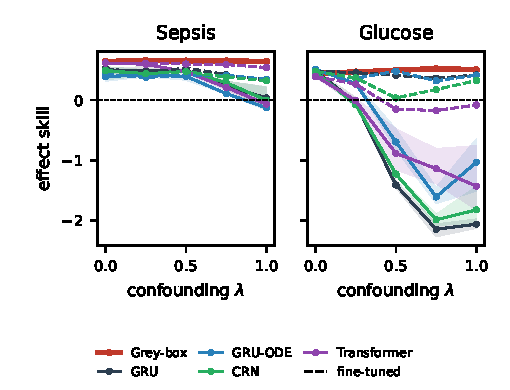
\includegraphics[width=\columnwidth]{v2_skill_vs_lambda.pdf}
\caption{Effect skill (raising the first drug 30\%) against confounding. Solid lines are trained models, with shading spanning the three seeds; dashed lines are the same baselines after fine-tuning on the randomised set. Below the black dashed line, a model's predicted effect is worse than predicting no effect.}
\label{fig:skill}
\end{figure}

\begin{table*}[t]
\centering
\begin{tabular}{lcccccc}
\toprule
 & \multicolumn{2}{c}{Effect skill $\uparrow$} & \multicolumn{4}{c}{$\lambda=1$} \\
\cmidrule(lr){2-3}\cmidrule(lr){4-7}
Model & $\lambda=0$ & $\lambda=1$ & CF RMSE $\downarrow$ & Fact.\ RMSE $\downarrow$ & Regret $\downarrow$ & CF cov. \\
\midrule
\multicolumn{7}{l}{\emph{Sepsis} (fixed best dose: regret 5.9)} \\
{\bfseries\boldmath Grey-box (ours)} & {\bfseries\boldmath 0.64\,$\pm$\,0.01} & {\bfseries\boldmath 0.64\,$\pm$\,0.00} & {\bfseries\boldmath 0.38\,$\pm$\,0.01} & {\bfseries\boldmath 0.33\,$\pm$\,0.02} & {\bfseries\boldmath 1.7} & {\bfseries\boldmath 0.79} \\
PK/PD only (ablation) & 0.64\,$\pm$\,0.00 & 0.63\,$\pm$\,0.00 & 0.39\,$\pm$\,0.00 & 0.34\,$\pm$\,0.01 & 1.5 & 0.80 \\
GRU & 0.49\,$\pm$\,0.04 & 0.03\,$\pm$\,0.17 & 0.63\,$\pm$\,0.00 & 0.21\,$\pm$\,0.00 & 8.8 & 0.61 \\
\quad + fine-tuned & 0.52\,$\pm$\,0.05 & 0.33\,$\pm$\,0.02 & 0.40\,$\pm$\,0.00 & 0.35\,$\pm$\,0.01 & 2.2 & 0.77 \\
GRU, IPW-weighted & 0.50\,$\pm$\,0.03 & $-$0.03\,$\pm$\,0.21 & 0.59\,$\pm$\,0.01 & 0.24\,$\pm$\,0.01 & 10.3 & 0.61 \\
GRU-ODE & 0.39\,$\pm$\,0.07 & $-$0.13\,$\pm$\,0.04 & 0.62\,$\pm$\,0.01 & 0.25\,$\pm$\,0.01 & 13.5 & 0.56 \\
\quad + fine-tuned & 0.42\,$\pm$\,0.10 & 0.34\,$\pm$\,0.01 & 0.42\,$\pm$\,0.02 & 0.36\,$\pm$\,0.02 & 2.4 & 0.72 \\
CRN & 0.47\,$\pm$\,0.12 & 0.00\,$\pm$\,0.20 & 0.66\,$\pm$\,0.01 & 0.22\,$\pm$\,0.01 & 9.2 & 0.60 \\
\quad + fine-tuned & 0.49\,$\pm$\,0.13 & 0.32\,$\pm$\,0.07 & 0.40\,$\pm$\,0.01 & 0.35\,$\pm$\,0.02 & 2.3 & 0.77 \\
Transformer & 0.61\,$\pm$\,0.01 & $-$0.07\,$\pm$\,0.07 & 0.57\,$\pm$\,0.03 & 0.23\,$\pm$\,0.03 & 10.7 & 0.66 \\
\quad + fine-tuned & 0.61\,$\pm$\,0.01 & 0.54\,$\pm$\,0.02 & 0.41\,$\pm$\,0.01 & 0.34\,$\pm$\,0.01 & 2.3 & 0.78 \\
\multicolumn{7}{l}{\emph{Glucose} (fixed best dose: regret 25.4)} \\
{\bfseries\boldmath Grey-box (ours)} & {\bfseries\boldmath 0.45\,$\pm$\,0.02} & {\bfseries\boldmath 0.50\,$\pm$\,0.00} & {\bfseries\boldmath 0.88\,$\pm$\,0.02} & {\bfseries\boldmath 0.85\,$\pm$\,0.03} & {\bfseries\boldmath 20.4} & {\bfseries\boldmath 0.84} \\
PK/PD only (ablation) & 0.45\,$\pm$\,0.01 & 0.48\,$\pm$\,0.01 & 1.05\,$\pm$\,0.02 & 1.01\,$\pm$\,0.02 & 25.6 & 0.87 \\
GRU & 0.48\,$\pm$\,0.01 & $-$2.06\,$\pm$\,0.08 & 1.24\,$\pm$\,0.00 & 0.26\,$\pm$\,0.01 & 76.4 & 0.84 \\
\quad + fine-tuned & 0.48\,$\pm$\,0.01 & 0.41\,$\pm$\,0.02 & 1.01\,$\pm$\,0.02 & 0.99\,$\pm$\,0.03 & 21.8 & 0.77 \\
GRU, IPW-weighted & 0.48\,$\pm$\,0.01 & $-$1.80\,$\pm$\,0.31 & 1.27\,$\pm$\,0.04 & 0.34\,$\pm$\,0.07 & 69.1 & 0.77 \\
GRU-ODE & 0.51\,$\pm$\,0.01 & $-$1.03\,$\pm$\,0.44 & 1.26\,$\pm$\,0.04 & 0.56\,$\pm$\,0.23 & 77.9 & 0.81 \\
\quad + fine-tuned & 0.47\,$\pm$\,0.04 & 0.41\,$\pm$\,0.07 & 1.08\,$\pm$\,0.08 & 1.02\,$\pm$\,0.09 & 26.2 & 0.79 \\
CRN & 0.47\,$\pm$\,0.03 & $-$1.82\,$\pm$\,0.34 & 1.24\,$\pm$\,0.01 & 0.28\,$\pm$\,0.03 & 72.2 & 0.87 \\
\quad + fine-tuned & 0.48\,$\pm$\,0.01 & 0.32\,$\pm$\,0.06 & 1.06\,$\pm$\,0.06 & 1.00\,$\pm$\,0.09 & 25.5 & 0.74 \\
Transformer & 0.40\,$\pm$\,0.02 & $-$1.43\,$\pm$\,0.59 & 1.32\,$\pm$\,0.04 & 0.50\,$\pm$\,0.24 & 56.1 & 0.82 \\
\quad + fine-tuned & 0.39\,$\pm$\,0.02 & $-$0.08\,$\pm$\,0.58 & 1.20\,$\pm$\,0.13 & 0.93\,$\pm$\,0.16 & 33.0 & 0.76 \\
\bottomrule
\end{tabular}

\caption{Our model is in bold. Effect skill under randomised ($\lambda=0$) and fully confounded ($\lambda=1$) training data, and the other metrics at $\lambda=1$. Arrows show which direction is better. ``+ fine-tuned'' is the baseline above it after fine-tuning on the 100 randomised trajectories. CF and factual RMSE are normalised, and factual RMSE uses the same horizon as the counterfactual metrics. Regret: how much further from target the model's chosen dose lands than the best dose; the fixed-dose regret is the bar to beat. CF cov.: worst coverage of 90\% intervals when doses are changed. All values are after calibration.}
\label{tab:main}
\end{table*}

\paragraph{Confounding breaks all four baselines, and factual error hides it.} With randomised data every model recovers the effects: effect skill is 0.39--0.64 on sepsis and 0.40--0.51 on glucose, and the grey-box model is no better than the best baseline on glucose (Table~\ref{tab:main}). As $\lambda$ rises, baseline effect skill falls (Figure~\ref{fig:skill}). On glucose it is already at or below zero for GRU, CRN and the Transformer at $\lambda=0.25$, and between $-0.70$ and $-1.41$ for all four at $\lambda=0.5$: these models predict that more basal insulin raises glucose. On sepsis it reaches $-0.13$ to $0.03$ at $\lambda=1$. Over the same range their factual error falls, from 0.71--0.74 to 0.26--0.56 on glucose, while their error on randomised patients nearly doubles. The models have learned to read severity from the dose.

\paragraph{Wrong effects lead to wrong decisions.} At $\lambda=1$, a dose chosen by a baseline leaves glucose 56--78 mg/dL further from target than the best dose, against 25 for giving everyone the same dose, and MAP 8.8--13.5 mmHg further, against 5.9. Baselines also stop foreseeing danger: glucose hazard recall is at most 0.01 for every baseline from $\lambda=0.5$, and sepsis recall falls from 0.87--0.89 to 0.14--0.21. Conformal calibration gives them intervals that cover the factual data, but only by multiplying their standard deviations by 3.9--8.2 on glucose, and when doses are changed their sepsis coverage is still 0.56--0.66.

\paragraph{The grey-box model keeps its effect skill.} Its effect skill is flat across $\lambda$: 0.64--0.66 on sepsis and 0.45--0.52 on glucose. At $\lambda=1$ its dosing beats the fixed dose on both simulators (regret 1.7 against 5.9, and 20.4 against 25.4), its sepsis hazard recall is 0.79, and its CF RMSE is 0.38 against 0.57--0.66 on sepsis and 0.88 against 1.24--1.32 on glucose. Most of this does not come from the multipliers: before they were fitted, effect skill at $\lambda=1$ was already 0.51 on sepsis and 0.45 on glucose. They mainly corrected NE, whose effect confounding had shrunk (sensitivity 0.62 before, 0.94 after, with $\kappa_{\mathrm{NE}}=1.57$). The price is factual accuracy under confounding: 0.33 against 0.21--0.25 on sepsis and 0.85 against 0.26--0.56 on glucose, because the model does not use the dose as a clue to severity. At $\lambda=0$ its factual error matches the baselines (0.73 against 0.71--0.74 on glucose).

\paragraph{100 randomised patients rescue most baselines, and the grey-box model stays ahead by less.} Fine-tuning has little effect at $\lambda=0$ but a large one under confounding. At $\lambda=1$, baseline effect skill rises to 0.32--0.54 on sepsis (from $-0.13$ to $0.03$) and to 0.32--0.41 on glucose for GRU, GRU-ODE and CRN (from $-2.06$ to $-1.03$). The fine-tuned Transformer stays negative on glucose ($-0.08\pm0.58$). Regret drops from 8.8--13.5 to 2.2--2.4 on sepsis, and from 56--78 to 21.8--33.0 on glucose. These are large gains, and they show that a large part of the benefit comes from having randomised patients at all.

The grey-box model still has the better mean at $\lambda=1$ on effect skill (0.64 against at most 0.54 on sepsis; 0.50 against at most 0.41 on glucose), regret (1.7 against 2.2--2.4; 20.4 against 21.8--33.0), CF RMSE (0.38 against 0.40--0.42; 0.88 against 1.01--1.20) and hazard recall (0.79 against 0.70--0.76; 0.49 against 0.02--0.29). With 3 seeds, the grey-box model's worst seed beats every fine-tuned baseline's best seed on effect skill, regret and CF RMSE on both simulators, and a permutation test across the four confounded settings finds it better in 22 of 24 comparisons after Holm correction (not glucose regret against fine-tuned GRU and GRU-ODE; Table~\ref{tab:stats}). Two tests specified in advance, on 10 fresh seeds each, at $\lambda=1$ and $\lambda=0.5$, confirm all 40 one-sided comparisons of each (4 fine-tuned baselines; effect skill, regret, CF RMSE, open- and closed-loop planning regret; Holm-corrected $p\le0.003$ at $\lambda=1$ and $\le0.045$ at $\lambda=0.5$; Appendix~\ref{sec:confirm}), though the seeds overlap on regret. Hazard recall on sepsis overlaps. Fine-tuned baselines also lose their factual advantage: on glucose at $\lambda=1$ their factual RMSE rises from 0.26--0.56 to 0.93--1.02, which is worse than the grey-box model's 0.85. Two differences matter more than the averages. On glucose at $\lambda\ge0.5$, the fine-tuned CRN and Transformer still predict the wrong direction for some patients (right for 0.49--0.98 of them, for the worse drug), and the grey-box model cannot do so by construction.

\paragraph{Inverse weighting does not help when the confounder is hidden.} The IPW-weighted GRU behaves like the plain GRU (Table~\ref{tab:main}). At $\lambda=1$ its effect skill is $-0.03$ on sepsis and $-1.80$ on glucose (GRU: 0.03 and $-2.06$), and it doses worse than the fixed dose. It helps only at $\lambda=0.25$ on glucose (0.22 against $-0.04$), where the recorded glucose still says much about the hidden severity. Extreme weights are not the reason: a version closer to RMSN, which weights only the doses inside the prediction window and truncates each step's weight at its 1st and 99th percentiles, rarely reaches the cap (at most 6\% of training windows) and fails the same way (glucose effect skill $-1.25$ to $-2.32$ at $\lambda\ge0.5$). Nor does giving either version the true severity (oracle IPW) fix it (glucose effect skill $-1.28$ and $-1.58$ at $\lambda=1$; Appendix~\ref{sec:ipw}).

\paragraph{The same ranking holds when planning over hours.} In multi-step planning at $\lambda=1$ (Table~\ref{tab:planning}, Appendix), the grey-box model's worst seed beats every seed of every baseline on both simulators, in open and closed loop (seeds 0--4). Re-planning on new readings helps every model that was not broken: grey-box regret falls from 1.59 to 0.71 on sepsis (fine-tuned baselines: 0.98--1.37) and from 5.57 to 4.26 on glucose (5.58--14.11; fixed schedule 5.71 and 8.07). The unadjusted and IPW-weighted baselines plan worse than the fixed schedule on glucose by a factor of about four, and re-planning does not rescue them. The PK/PD-only model plans best on sepsis (0.60 closed loop) but worse than the grey-box model on glucose (5.16).

\begin{figure}[t]
\centering
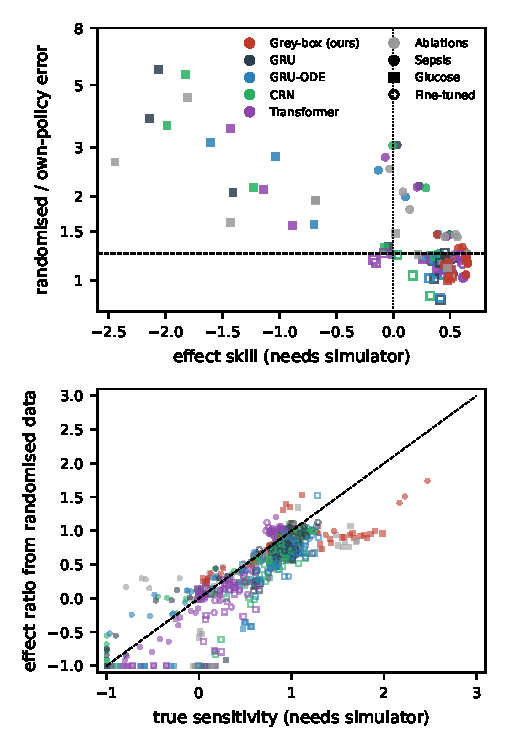
\includegraphics[width=\columnwidth]{v2_audit.pdf}
\caption{Top: one point per configuration (model, simulator, $\lambda$, ablation or misspecified prior), averaged over seeds; hollow points are fine-tuned baselines. Error on randomised patients divided by error on the model's own policy, with the 1.25 pass mark dashed. Bottom: one point per trained model and drug. The effect ratio from the effect test on 72 randomised patients, against the true sensitivity (1 is correct; values clipped to $[-1,3]$). The $x$ axes need a simulator, and the $y$ axes do not.}
\label{fig:audit}
\end{figure}

\begin{table}[t]
\centering
\resizebox{\columnwidth}{!}{\begin{tabular}{lccccc}
\toprule
 & \multicolumn{2}{c}{All 312 models} & \multicolumn{2}{c}{Fine-tuned (120)} & \\
\cmidrule(lr){2-3}\cmidrule(lr){4-5}
Check & caught & false al. & caught & false al. & AUC \\
\midrule
Direction & 105/110 & 25/202 & 11/13 & 16/107 & 0.97 \\
Randomised gap & 98/110 & 29/202 & 5/13 & 11/107 & 0.92 \\
Randomised coverage & 3/110 & 3/202 & 3/13 & 3/107 & 0.28 \\
\textbf{Effect test (new)} & 108/110 & 80/202 & 12/13 & 42/107 & 0.95 \\
\midrule
First three & 105/110 & 50/202 & 11/13 & 26/107 & -- \\
All four & 109/110 & 93/202 & 13/13 & 51/107 & -- \\
\bottomrule
\end{tabular}
}
\caption{Deployable checks on every trained model (312 = 104 configurations $\times$ 3 seeds). Caught: seriously broken models flagged. False al.: models flagged that are not seriously broken. AUC: how well the check's continuous score ranks broken above sound models (0.5 is chance).}
\label{tab:audit}
\end{table}

\paragraph{Testing whether errors depend on the dose catches broken models without a simulator.} We now judge each trained model separately and call it seriously broken if any effect skill of \emph{either} drug is negative or its dosing is worse than the fixed dose. 110 of the 312 models are (Table~\ref{tab:audit}). The direction and gap checks catch most broken models trained on the records, but the gap fails after fine-tuning. It catches 5 of the 13 broken fine-tuned models, and among fine-tuned models it ranks broken above sound no better than chance (AUC 0.51). The gap detects a model that reads severity from the dose. Fine-tuning removes that habit without making the effects correct, and on glucose at $\lambda=1$ some broken fine-tuned models have a gap below 1. The effect test catches 12 of the 13, and the four checks together catch all 13. Over all models it catches 108 of 110 and ranks them about as well as the direction check (AUC 0.95 against 0.97), and unlike the direction check it also says something about the grey-box model, whose direction is fixed. Randomised coverage is useless here (AUC 0.28), probably because conformal calibration on randomised patients already widens every model's intervals enough. Averaged over seeds, as in our earlier analysis, the four checks catch all 37 broken configurations.

\paragraph{What the test misses, and what it flags.} The one broken model no check catches is a single seed of the grey-box model with $\Emax$ four times too large. The cost is false alarms: the test flags 80 of the 202 models that are not seriously broken, against 50 for the first three checks together. Many of these models are still wrong, just not badly enough to count as broken. In analyses we added afterwards, 46 of the 80 have a drug whose true sensitivity is below 0.5 or above 2, against 2 of the 122 models the test passes. Leaving out the bolus, whose sensitivity uses an unrealistic dose change, 67 of the 80 have a drug off by more than 1.5-fold, and of the 115 models whose effects are all within 1.5-fold the test flags 13. A stricter cut-off trades a little sensitivity for far fewer flags: at 99\% instead of 95\% (approximating the bootstrap interval by its s.d.) it catches 103 of the 110 broken models and flags 37 of the other 202. The test also says which drug is off and by how much: its effect ratio tracks the true sensitivity ($r=0.78$ over 624 model--drug pairs; Figure~\ref{fig:audit}, bottom). It flags the grey-box model itself on sepsis in 4 of 6 runs at $\lambda\ge0.75$, every time for fluids, with ratio 0.36--0.48 against a true 0.23--0.58: the weakness described in the Discussion. It does not see the grey-box bolus over-estimate (ratio about 0.9 against a true 1.3--2.0), which appears only under sustained bolus dosing that the randomised patients never receive.

\paragraph{How far the test can be trusted.} A cut-off chosen on one simulator works on the other. Choosing the test-statistic threshold on sepsis and applying it to glucose gives sensitivity 0.83 and specificity 0.95, and the reverse gives 0.80 and 0.92. The test needs enough patients: on random subsets of 18, 36 and 54 of the 72 it catches 72\%, 90\% and 96\% of broken models, while flagging 24--34\% of the others. The checks miss milder failures such as low hazard recall or a wrong time course.

\begin{table}[t]
\centering
\resizebox{\columnwidth}{!}{\begin{tabular}{lcccccc}
\toprule
 & \multicolumn{3}{c}{Sepsis} & \multicolumn{3}{c}{Glucose} \\
\cmidrule(lr){2-4}\cmidrule(lr){5-7}
Variant & Skill & Dir. & Gap & Skill & Dir. & Gap \\
\midrule
{\bfseries\boldmath Grey-box (ours)} & {\bfseries\boldmath 0.65} & {\bfseries\boldmath 1.00} & {\bfseries\boldmath 1.25} & {\bfseries\boldmath 0.52} & {\bfseries\boldmath 1.00} & {\bfseries\boldmath 1.03} \\
+ residual $R$ & 0.65 & 1.00 & 1.25 & 0.50 & 1.00 & 1.06 \\
Raw-action residual & 0.55 & 0.12 & 1.46 & $-$0.69 & 0.48 & 1.93 \\
Action leak & 0.56 & 0.23 & 1.43 & $-$0.68 & 0.56 & 1.94 \\
Effect into latent & 0.15 & 0.36 & 1.80 & 0.02 & 0.76 & 1.48 \\
\bottomrule
\end{tabular}
}
\caption{Ablations at $\lambda=0.75$, each changing one design choice. Our model is in bold. Skill: effect skill. Dir.: worst share of patients with the right effect direction. Gap: error on randomised patients divided by error on the model's own policy (pass mark: 1.25).}
\label{tab:ablation}
\end{table}

\paragraph{The route of the dose matters more than having a PK/PD block.} All ablations in Table~\ref{tab:ablation} keep the PK/PD block. Letting the raw action reach the latent through an unconstrained residual, or giving it to $f_\phi$ as an input, turns glucose effect skill negative ($-0.69$, $-0.68$) and makes the predicted effect of one sepsis drug point the wrong way for most patients. Feeding the PD effect into $f_\phi$ instead of adding it with a fixed sign removes the guarantee, and effect skill falls to 0.15 and 0.02. The deployable gates flag each of these variants. A monotone correction $R_c(C)$ on top of the PD curve, which can only add to an effect, changed nothing measurable, so we leave it out.

\paragraph{Pharmacology sets the effects; the learned course makes them usable on glucose.} A PK/PD-only variant (added after the main runs) has no learned untreated course: after the context, the latent stays where the filter left it. Its effect skill equals the grey-box model's at every $\lambda$ on both simulators (Table~\ref{tab:main}), so the effect estimates come from the pharmacology. On sepsis, whose untreated course is slow, it is as good or slightly better on every metric. At $\lambda=1$ its regret is 1.5 against 1.7, hazard recall 0.83 against 0.79, and its fluid effect is much closer to the truth (sensitivity 0.80 against 0.44), so its worst time-course ratio passes the gate (0.79 against 0.44). Here the learned course adds nothing and absorbs part of the fluid effect. On glucose, where meals drive the course, it doses worse. Its regret margin falls from 11.4 to 5.2 at $\lambda=0$ and to $-0.2$ at $\lambda=1$ (against 4.9), which is worse than the fixed dose, and its hazard recall at $\lambda=1$ falls from 0.49 to 0.20. Correct effects are not enough for good decisions; the model must also follow the patient's course without treatment.

\paragraph{Wrong priors cost effect size or timing, not direction.} Scaling $\Emax$ or the Hill coefficient of both drugs by up to fourfold at $\lambda=0.75$ keeps the direction in every run and effect skill positive (sepsis 0.39--0.63, glucose 0.45--0.52), and on glucose dosing beats the fixed dose in all 24 runs. Calibration repairs moderate errors but not a fourfold under-estimate of NE (sensitivity 0.49); a variant that also fits one $\mathrm{EC}_{50}$ multiplier per drug largely does. Priors of the wrong form (insulin without its depot or its delay; a delay the sepsis simulator does not have) cost more: glucose effect skill falls to 0.32--0.41, though dosing still beats the fixed dose, and the effect test, which judges the average size of an effect and not its timing, flags 1 of these 9 models (a version that tests each third of the window flags 3). Details are in Appendix~\ref{sec:misspec}.

\paragraph{The bolus over-estimate comes from how we measured it.} Our sensitivity metric raises a drug at every step of the window. For boluses that means extra insulin every 5 minutes for 6 h, which never happens in the data. Under bolus changes that do occur, the same grey-box models are close or slightly low: 0.75--0.84 of the true effect for one extra bolus and 0.88--1.01 with the recorded boluses raised by 30\%, against 1.57--1.75 on our metric (correct prior, all $\lambda$). The effect test, which also sees only realistic doses, agrees with the single-bolus ratio within a median factor of 1.2, against 1.8 for our metric. Measured this way at $\lambda=1$, the grey-box model's lead grows: it gets 0.83 of the effect of one extra bolus, the fine-tuned GRU, GRU-ODE and CRN 0.43--0.51, the fine-tuned Transformer 0.02, and the unadjusted baselines 0.01--0.09. An effect metric must use dose changes that a clinician could make.

\paragraph{25 randomised patients suffice for the grey-box model, but not for fine-tuning.} With only 25 or 50 randomised trajectories, the grey-box model keeps its effect skill (sepsis 0.63--0.64, glucose 0.50) and beats the fixed dose, while all three fine-tuned baselines dose glucose worse than the fixed dose (Appendix~\ref{sec:size}). When the 50 randomised patients are the least sick rather than a random half, the grey-box model keeps its effect skill but beats the fixed glucose dose in only 7 of 10 seeds, and the fine-tuned baselines do far worse; when they are the sickest, the fine-tuned GRU nearly catches up on glucose (Appendix~\ref{sec:shift}).

\section{Discussion and Limitations}

Our results support three practical points. If the direction of a drug's effect is known with confidence, a world model should be unable to reverse it. Some randomised data should be used to set or correct effects, because under confounding it helped every model we tested and is the reason the baselines recover. And a model should be checked on randomised patients before use by testing whether its errors depend on the dose. In our runs this caught almost every broken model, fine-tuned ones included, and its effect ratio said which drug was wrong. Its flags are frequent, though, and a pass is not proof of correctness. Fixing the direction of an effect is not the same as estimating its size, and the grey-box model does not pass every gate.
\begin{itemize}
\item \emph{Fluids.} Its sepsis fluid effect is too small: sensitivity 0.72--0.75 at $\lambda\le0.5$ and 0.44 at $\lambda=1$, and its worst time-course ratio is 0.44--0.53 at $\lambda\ge0.75$, failing that gate. We traced two causes after the main runs (Appendix~\ref{sec:fluid}): the prior lacks the simulator's faster fluid leak in sicker patients, and the learned untreated course absorbs part of the effect (without it, sensitivity is 0.80 at $\lambda=1$). A refitted dose--response, a looser prior and state-dependent elimination each fail to fix it without costs elsewhere.
\item \emph{Boluses.} On glucose, its bolus effect is 1.6--1.8 times too large under sustained bolus dosing at every $\lambda$, but 0.75--0.84 of the true effect for a single extra bolus. It is accurate only for dose changes like those in the data.
\item \emph{Gates it fails.} Glucose hazard recall is 0.48--0.65 against a pass mark of 0.7. Every model fails it, even with randomised data (0.37--0.56), so it is probably too strict. Sepsis CF coverage is 0.79 against 0.8, always under the stop-all-drugs policy. A separate interval multiplier per rollout step does not fix it (0.79--0.80), because no calibration patient goes without drug.
\end{itemize}
More broadly, both environments are simulators, the sepsis one is not validated, and we have no result on real clinical data. The priors match the simulators, and the insulin prior was fitted to the simulator's own responses after a first version failed, which is a best case. The baselines are our own implementations with one setting each; our Transformer in particular may be under-tuned (its fine-tuned glucose effect skill stays negative), although on randomised data it learns the effects (effect skill 0.40 on glucose and 0.61 on sepsis, the best baseline there), so its failures come with confounding. We did not run the Causal Transformer \citep{melnychuk2022causal} or G-Net \citep{li2021gnet}, which adjust for recorded confounders and so would face the same hidden confounder (our baselines already predict forward under the changed doses, as G-Net's g-computation does, though without its sampling of future covariates). Two other ways to fine-tune, updating only the output layer or penalising distance from the trained weights (L2-SP), did no better than plain fine-tuning (Appendix~\ref{sec:ftvar}); other schemes might. Misspecification was tested at one $\lambda$, and wrong forms only for timing (a missing compartment or a wrong delay) and one dose--response family (linear), not for drug interactions. Dosing follows hidden severity alone; in real records it also follows recorded variables, which weighting methods can correct and which our benchmark does not test. Our propensity models are linear-Gaussian and do not capture the clipped, nonlinear dosing rule, which may explain part of the oracle-IPW failure. We assume known effect directions, which excludes drugs with mixed or state-dependent effects. Planning chooses among 27 schedules of one drug, not a continuous policy. The randomised set is a luxury that real data seldom offer, although the sets used here (18--100 patients) are the size of a pilot trial, far too small to train a model on; with 25 or 50 of them, fine-tuning the baselines was unreliable. Randomising a vasopressor or insulin dose is ethical only within a safe range, as in a dose-finding trial, and our randomised doses span the full range. Here 25 patients sufficed for the grey-box model, but whether quasi-randomised patients or natural experiments can replace them is open. The tables report effect skill and regret for the first drug of each simulator; the second drug's effect skill enters only the definition of a broken model. The effect test was designed after we saw the other checks fail, and all its results come from the same two simulators. It needs a randomised hold-out set, with 18 patients it misses over a quarter of broken models, it cannot judge effects of dose changes that the randomised patients never received, and it rarely sees effects with the wrong timing: testing each third of the prediction window separately flags 3 of 9 wrong-form models instead of 1, and catches no more broken ones (Appendix~\ref{sec:misspec}). Finally, most comparisons rest on 3 seeds; only those against the fine-tuned baselines at $\lambda=1$ and $0.5$ were confirmed on fresh seeds.

\section{Conclusion}

Trained on data confounded by indication, four standard sequence models learned drug effects worse than assuming no effect, and dosing by them was worse than a fixed dose, while their forecasts of the recorded data kept improving. Fine-tuning on 100 randomised patients repaired most of this; inverse weighting did not. A grey-box world model, which lets the dose act only through fixed-direction pharmacology and sets effect sizes on the same patients, kept useful effects, dosing and planning at every confounding level and stayed ahead of the fine-tuned baselines, at the cost of factual accuracy and with a fluid effect that is too small. A small randomised set can both correct models and, by testing whether errors depend on the dose, expose nearly all that are broken, though a pass does not prove a model right.

\paragraph{Code.} The simulators, data generation, all models, the effect test and the scripts that produce every table and figure are released at \url{https://github.com/ParamThakkar123/grey_wm} under the MIT licence.

\ifaaaikit
\bibliography{refs}
\else
\ifaaaikit\bibliographystyle{\aaaistyle}\else\bibliographystyle{plainnat}\fi
\bibliography{refs}
\fi

\clearpage
\appendix
\noindent\textbf{Guide to the appendices.} Much of what follows was added after the main runs (Appendix~\ref{sec:decisions} lists what was decided when). In brief: \ref{sec:size}, 25 randomised patients suffice for the grey-box model but not for fine-tuning; \ref{sec:misspec}, wrong priors cost effect size or timing, never direction, and the effect test sees size errors better than timing errors; \ref{sec:ftvar}, fine-tuning only the output layer or with L2-SP does no better than plain fine-tuning; \ref{sec:shift}, which patients are randomised matters for fine-tuning, and for the grey-box model's glucose dosing; \ref{sec:ipw}, no version of inverse weighting helps under strong confounding, even with the true severity or with few extreme weights; \ref{sec:fluid}, why the sepsis fluid effect is too small; \ref{sec:confirm}, the two tests on fresh seeds (80 of 80 hold); \ref{sec:planning}, the planning table; \ref{sec:decisions}, the order of decisions.

\section{Size of the Randomised Set}
\label{sec:size}

Given only the first 25 or 50 randomised trajectories (Table~\ref{tab:size}, Appendix), the grey-box model keeps its effect skill (sepsis 0.63--0.64, glucose 0.50) and beats the fixed dose at every size. The fine-tuned baselines keep positive effect skill on sepsis (0.09--0.43), but on glucose all three dose worse than the fixed dose with 25 or 50 patients (regret margin $-4.7$ to $-35.8$), and with 50 their effect skill is negative. That 50 is worse than 25 points to unstable fine-tuning on few patients rather than a trend; one CRN seed stopped after 50 steps with effect skill $-1.18$. On these models the effect test caught 15 of the 16 broken fine-tuned ones (the gap alone caught 7), while flagging 14 of the other 20. It flagged 3 of the 12 grey-box models, each for a sepsis fluid effect under-estimated by about half, which its effect ratio measured correctly (0.51--0.54, true 0.48--0.64).

\begin{table}[h]
\centering
\resizebox{\columnwidth}{!}{\begin{tabular}{llcccccc}
\toprule
 & & \multicolumn{3}{c}{Effect skill $\uparrow$} & \multicolumn{3}{c}{Regret margin $\uparrow$} \\
\cmidrule(lr){3-5}\cmidrule(lr){6-8}
 & Model & $n{=}25$ & $50$ & $100$ & $25$ & $50$ & $100$ \\
\midrule
{\bfseries\boldmath Sepsis} & {\bfseries\boldmath Grey-box (ours)} & {\bfseries\boldmath 0.63} & {\bfseries\boldmath 0.64} & {\bfseries\boldmath 0.64} & {\bfseries\boldmath 4.1} & {\bfseries\boldmath 4.2} & {\bfseries\boldmath 4.2} \\
 & GRU (no fine-tune) & 0.02 & 0.02 & 0.03 & $-$2.9 & $-$2.9 & $-$2.9 \\
 & GRU fine-tuned & 0.43 & 0.41 & 0.33 & 2.9 & 2.8 & 3.7 \\
 & GRU-ODE fine-tuned & 0.09 & 0.37 & 0.34 & 0.2 & 3.4 & 3.6 \\
 & CRN fine-tuned & 0.40 & 0.40 & 0.32 & 1.4 & 2.6 & 3.6 \\
\midrule
{\bfseries\boldmath Glucose} & {\bfseries\boldmath Grey-box (ours)} & {\bfseries\boldmath 0.50} & {\bfseries\boldmath 0.50} & {\bfseries\boldmath 0.50} & {\bfseries\boldmath 3.0} & {\bfseries\boldmath 5.4} & {\bfseries\boldmath 4.9} \\
 & GRU (no fine-tune) & $-$2.13 & $-$1.88 & $-$2.06 & $-$54.5 & $-$54.5 & $-$51.1 \\
 & GRU fine-tuned & 0.27 & $-$0.74 & 0.41 & $-$4.7 & $-$35.8 & 3.6 \\
 & GRU-ODE fine-tuned & 0.09 & $-$0.14 & 0.41 & $-$26.6 & $-$28.5 & $-$0.8 \\
 & CRN fine-tuned & 0.26 & $-$0.16 & 0.32 & $-$5.8 & $-$13.8 & $-$0.1 \\
\bottomrule
\end{tabular}
}
\caption{Size study at $\lambda=1$: models given only the first $n$ of the 100 randomised trajectories ($n=100$ is the main sweep), mean of 3 seeds. Our model is in bold. Effect skill under a sustained dose increase of the first drug, and regret margin: regret of the fixed best dose minus the model's regret (positive is better than the fixed dose). The unadjusted GRU uses the randomised set only for early stopping.}
\label{tab:size}
\end{table}

\section{Wrong Priors}
\label{sec:misspec}

\paragraph{Effect size still depends on the prior.} Table~\ref{tab:misspec} scales $\Emax$ by 0.25 to 4 or the Hill coefficient by 0.5 or 2. Effect direction is preserved in every run, and effect skill stays positive (0.39--0.63, against 0.65 with the correct prior). Calibration repairs moderate under-estimates ($\Emax\times0.5$: NE sensitivity 0.53 to 0.83; $h\times0.5$: 0.47 to 0.75) but not a fourfold one (0.38 to 0.49), and it does not shrink a fourfold over-estimate (1.24 to 1.28). The prior on $\kappa$ is not what stops it: widening it threefold changes no sensitivity or skill by more than 0.02. Letting calibration also fit one $\mathrm{EC}_{50}$ multiplier per drug does better on wrong priors: it fixes the fourfold over-estimate (NE sensitivity 0.93, fluid 2.29 to 1.00, effect skill 0.47 to 0.61) and moves the under-estimates closer (NE 0.65, 0.93 and 0.98, against 0.49, 0.83 and 0.75), while changing effect skill by at most 0.02 with the correct prior (Table~\ref{tab:recal}, Appendix). We found both after the main runs, so the tables keep the original calibration. The randomised gap flags the three priors that are too low (1.31--1.46) but not those that are too high (1.20--1.22).

\paragraph{On glucose, wrong priors cost little.} The same errors on glucose, plus $k_e\times0.5$ or 2 (Table~\ref{tab:misspec_glucose}, Appendix), keep the direction in all 24 runs, effect skill at 0.45--0.52 (0.52 with the correct prior) and dosing better than the fixed dose (regret margin 2.8--6.6, against 5.4). Unlike on sepsis, calibration repairs a fourfold under-estimate of $\Emax$ (bolus sensitivity 0.63 to 1.05) and pulls a fourfold over-estimate down (2.98 to 1.80). It keeps the 1.6-fold bolus over-estimate of the correct prior, though, and raises it for $h\times2$ (1.23 to 2.24). The gap stays at 0.96--1.13, and the effect test flags 1 of the 24 models, with bolus effect ratios of 0.54--1.17. As the next paragraph shows, these over-estimates exist only under sustained bolus dosing. With wrong priors, the single-bolus ratio is 0.28--0.96, so $h\times2$ is in fact a fourfold under-estimate of one bolus.

\paragraph{A prior of the wrong form costs more.} Scaling parameters keeps the form of the prior right. After the main runs we also gave the model wrong forms at $\lambda=0.75$, 3 seeds each: insulin without its depot under the skin (one compartment too few), insulin acting without delay, and on sepsis an effect delay (1/h) for both drugs that the simulator does not have. The direction is still fixed, and calibration still sets the size of the basal effect (sensitivity 1.13 and 1.08 against 0.99), but the timing is wrong and effect skill falls. On glucose it falls from 0.52 to 0.41 without the depot and to 0.32 without the delay, and dosing still beats the fixed dose by less (regret margin 2.9 and 1.3, against 5.4). On sepsis the added delay leaves effect skill and dosing almost unchanged (0.60 against 0.65; margin 4.4 against 4.5) but halves the fluid effect again (0.28) and ruins the time course (worst ratio 0.20). The effect test flags none of the six glucose models and one of the three sepsis models (for fluids): it judges the average size of an effect over the window, not its timing. It flags none of the 30 PK/PD-only models.

\paragraph{A timing-aware effect test helps little.} After these results we defined, before computing it (\texttt{notes/}), a version of the effect test that cuts each prediction window into three equal parts and regresses each part's error on the doses given up to its end, flagging a model if any part's slope differs from zero (Bonferroni over the three parts). On the 312 models of the main audit it catches 107 of the 110 broken ones and flags 77 of the other 202 (the effect test: 108 and 80; either test: 108 and 87). It flags 3 of the 9 wrong-form models (the effect test 1), none of the 6 linear ones, none of the 30 PK/PD-only ones and 4 of the 15 fluid-only elimination models (the effect test 5). Timing errors that cancel over a window remain hard to see from 72 randomised patients.

A wrong dose--response family (linear instead of $\Emax$, same slope at low concentration; 3 seeds per simulator, run on the last day) matters little on glucose (effect skill 0.51, margin 5.3; the bolus effect is over-estimated, 1.97) but more on sepsis, where doses reach the saturating part of the curve: effect skill falls to 0.43 (margin 3.8) and the effects are over-estimated (fluid 1.52, NE 1.20). The effect test flags none of these six models (largest $z$ 1.9), so a 1.5-fold over-estimate can pass it.

\begin{table}[h]
\centering
\resizebox{\columnwidth}{!}{\begin{tabular}{lccccc}
\toprule
 & \multicolumn{2}{c}{NE sensitivity} & & & \\
\cmidrule(lr){2-3}
Assumed prior & raw & calibrated & $\kappa_{\mathrm{NE}}$ & Skill & Gap \\
\midrule
{\bfseries\boldmath correct} & {\bfseries\boldmath 0.70} & {\bfseries\boldmath 0.97} & {\bfseries\boldmath 1.45} & {\bfseries\boldmath 0.65} & {\bfseries\boldmath 1.25} \\
$E_{\max}\times0.25$ & 0.38 & 0.49 & 1.45 & 0.39 & 1.46 \\
$E_{\max}\times0.5$ & 0.53 & 0.83 & 1.69 & 0.61 & 1.32 \\
$E_{\max}\times2$ & 0.92 & 1.08 & 1.20 & 0.63 & 1.22 \\
$E_{\max}\times4$ & 1.24 & 1.28 & 1.04 & 0.47 & 1.20 \\
$h\times0.5$ & 0.47 & 0.75 & 1.72 & 0.58 & 1.31 \\
$h\times2$ & 0.71 & 0.96 & 1.35 & 0.52 & 1.22 \\
\bottomrule
\end{tabular}
}
\caption{Wrong priors on sepsis, $\lambda=0.75$, applied to both drugs. The correct prior is in bold. NE sensitivity (1 is correct) before and after calibration, the fitted multiplier, effect skill and randomised gap.}
\label{tab:misspec}
\end{table}


\begin{table}[h]
\centering
\resizebox{\columnwidth}{!}{\begin{tabular}{lcccccc}
\toprule
 & \multicolumn{2}{c}{Bolus sensitivity} & & & & \\
\cmidrule(lr){2-3}
Assumed prior & raw & calibrated & $\kappa_{\mathrm{bolus}}$ & $\kappa_{\mathrm{basal}}$ & Skill & Gap \\
\midrule
{\bfseries\boldmath correct} & {\bfseries\boldmath 1.64} & {\bfseries\boldmath 1.57} & {\bfseries\boldmath 0.95} & {\bfseries\boldmath 1.21} & {\bfseries\boldmath 0.52} & {\bfseries\boldmath 1.03} \\
$E_{\max}\times0.25$ & 0.63 & 1.05 & 1.66 & 4.87 & 0.49 & 1.03 \\
$E_{\max}\times0.5$ & 1.03 & 1.15 & 1.10 & 2.16 & 0.52 & 1.07 \\
$E_{\max}\times2$ & 2.19 & 1.81 & 0.83 & 0.83 & 0.52 & 1.05 \\
$E_{\max}\times4$ & 2.98 & 1.80 & 0.62 & 0.71 & 0.51 & 0.96 \\
$h\times0.5$ & 1.00 & 0.94 & 0.94 & 0.85 & 0.49 & 1.08 \\
$h\times2$ & 1.23 & 2.24 & 1.76 & 5.25 & 0.45 & 1.04 \\
$k_e\times0.5$ & 1.65 & 1.34 & 0.81 & 0.86 & 0.47 & 1.13 \\
$k_e\times2$ & 1.36 & 1.40 & 1.02 & 2.00 & 0.49 & 0.98 \\
\bottomrule
\end{tabular}
}
\caption{Wrong priors on glucose, $\lambda=0.75$, applied to both drugs, mean of 3 seeds. The correct prior is in bold. Bolus sensitivity (1 is correct) before and after calibration, the fitted multipliers, effect skill and randomised gap.}
\label{tab:misspec_glucose}
\end{table}

\begin{table}[h]
\centering
\resizebox{\columnwidth}{!}{\begin{tabular}{lccccccccc}
\toprule
 & \multicolumn{4}{c}{Sepsis, $\lambda=1$} & \multicolumn{3}{c}{Sepsis, $E_{\max}\times4$, $\lambda=0.75$} & \multicolumn{2}{c}{Glucose, $\lambda=1$} \\
\cmidrule(lr){2-5}\cmidrule(lr){6-8}\cmidrule(lr){9-10}
Calibration & Skill & Fluid & CF cov. & Course & Skill & NE & Fluid & Skill & CF cov. \\
\midrule
Paper & 0.64 & 0.44 & 0.79 & 0.44 & 0.47 & 1.28 & 2.29 & 0.50 & 0.84 \\
Per-step $s$ & 0.64 & 0.44 & 0.79 & 0.44 & -- & -- & -- & 0.50 & 0.84 \\
$+\mathrm{EC}_{50}$ & 0.63 & 0.47 & 0.79 & 0.47 & 0.61 & 0.93 & 1.00 & 0.50 & 0.84 \\
Loose prior & 0.64 & 0.43 & 0.79 & 0.43 & 0.47 & 1.28 & 2.29 & 0.50 & 0.84 \\
\bottomrule
\end{tabular}
}
\caption{Post hoc calibration variants on the saved grey-box models (no retraining), mean of 3 seeds. Paper: the calibration used in all other tables (it reproduces their numbers). Per-step $s$: one conformal sd multiplier per rollout step. $+\mathrm{EC}_{50}$: one $\mathrm{EC}_{50}$ multiplier per drug fitted with $\kappa$. Loose prior: prior sd on $\log\kappa$ 1.5 instead of 0.5. Fluid and NE: sensitivity (1 is correct); Course: worst time-course ratio; CF cov.: worst CF coverage.}
\label{tab:recal}
\end{table}

\begin{table}[h]
\centering
\resizebox{\columnwidth}{!}{\begin{tabular}{llccc}
\toprule
 & Fine-tuned & Effect skill & Regret & CF RMSE \\
\midrule
Sepsis & GRU & 0.21$^{*}$ & $-$0.18$^{*}$ & $-$0.01$^{*}$ \\
 &  & {\scriptsize[0.19, 0.24]} & {\scriptsize[$-$0.29, $-$0.09]} & {\scriptsize[$-$0.01, $-$0.01]} \\[2pt]
 & GRU-ODE & 0.26$^{*}$ & $-$0.51$^{*}$ & $-$0.03$^{*}$ \\
 &  & {\scriptsize[0.25, 0.28]} & {\scriptsize[$-$0.62, $-$0.40]} & {\scriptsize[$-$0.04, $-$0.02]} \\[2pt]
 & CRN & 0.25$^{*}$ & $-$0.36$^{*}$ & $-$0.02$^{*}$ \\
 &  & {\scriptsize[0.22, 0.28]} & {\scriptsize[$-$0.43, $-$0.29]} & {\scriptsize[$-$0.02, $-$0.01]} \\[2pt]
 & Transformer & 0.06$^{*}$ & $-$0.35$^{*}$ & $-$0.01$^{*}$ \\
 &  & {\scriptsize[0.06, 0.07]} & {\scriptsize[$-$0.51, $-$0.19]} & {\scriptsize[$-$0.02, $-$0.01]} \\[2pt]
\midrule
Glucose & GRU & 0.08$^{*}$ & $-$1.11 & $-$0.07$^{*}$ \\
 &  & {\scriptsize[0.06, 0.11]} & {\scriptsize[$-$2.33, $-$0.02]} & {\scriptsize[$-$0.08, $-$0.05]} \\[2pt]
 & GRU-ODE & 0.10$^{*}$ & $-$4.78 & $-$0.08$^{*}$ \\
 &  & {\scriptsize[0.03, 0.18]} & {\scriptsize[$-$11.79, $-$0.62]} & {\scriptsize[$-$0.11, $-$0.05]} \\[2pt]
 & CRN & 0.27$^{*}$ & $-$10.99$^{*}$ & $-$0.10$^{*}$ \\
 &  & {\scriptsize[0.15, 0.40]} & {\scriptsize[$-$16.81, $-$4.53]} & {\scriptsize[$-$0.13, $-$0.08]} \\[2pt]
 & Transformer & 0.53$^{*}$ & $-$18.64$^{*}$ & $-$0.27$^{*}$ \\
 &  & {\scriptsize[0.34, 0.74]} & {\scriptsize[$-$24.53, $-$13.06]} & {\scriptsize[$-$0.32, $-$0.22]} \\[2pt]
\bottomrule
\end{tabular}
}
\caption{Grey-box model minus each fine-tuned baseline, averaged over $\lambda\in\{0.25,0.5,0.75,1\}$ and 3 seeds. Positive differences in effect skill and negative ones in regret and CF RMSE favour the grey-box model. Brackets: 95\% bootstrap interval over seeds. $^{*}$: one-sided exact permutation test (seeds shuffled between the two models within each $\lambda$, 160\,000 permutations), Holm-corrected over the 24 tests, $p<0.05$. Code: \texttt{scripts/stats\_tests.py}.}
\label{tab:stats}
\end{table}

\section{Stronger Fine-Tuning}
\label{sec:ftvar}

Plain fine-tuning updates every weight with no regulariser, so a better scheme might close the gap. After the main runs we tried two, at $\lambda\in\{0.5,1\}$, with seeds 0--9 for the GRU, GRU-ODE and CRN at $\lambda=1$ and seeds 0--2 otherwise, and with everything else as in plain fine-tuning: (i) \emph{output layer only}, which updates only the decoder that maps the latent state to observations; (ii) \emph{L2-SP}, which updates every weight with a penalty $\tfrac{\alpha}{2}\lVert w-w_{\mathrm{trained}}\rVert^2$, $\alpha$ chosen from $\{0.001,0.01,0.1,1\}$ on the same 20 stopping trajectories.

Updating the output layer only is much worse on glucose: every baseline then doses worse than the fixed dose (mean regret margin $-1.6$ to $-63.7$, against $-36.7$ to $6.6$ for plain fine-tuning; at $\lambda=1$ none of the 30 GRU, GRU-ODE and CRN runs beats the fixed dose), and on sepsis at $\lambda=1$ its margin falls from 3.4--3.7 to $-0.4$--1.2. The confounded part of these models is in the learned dynamics, not in the output layer. L2-SP ends close to plain fine-tuning on average, usually with a small $\alpha$: mean effect skill differs by at most 0.14 and mean regret margin by at most 6.6 (the Transformer on glucose at $\lambda=1$, $-14.3$ against $-7.7$). Its largest gains are on glucose: CRN at $\lambda=0.5$ ($-15.2$ against $-21.0$, still far worse than the fixed dose) and the GRU at $\lambda=1$ (0.7 against $-3.8$), where the gain comes mostly from one seed on which plain fine-tuning failed (39.6 better; on the other nine seeds the two differ by at most 5.2). With L2-SP the GRU, GRU-ODE and CRN beat the fixed glucose dose in 8, 4 and 6 of 10 seeds at $\lambda=1$, against 8, 5 and 8 with plain fine-tuning; the grey-box model does so in all 10, and has a higher glucose effect skill than the L2-SP baseline on 29 of these 30 seed pairs and the higher margin on 29. Neither scheme reaches the grey-box model's mean effect skill on any of the 16 baseline--simulator--$\lambda$ combinations, and with either scheme the Transformer still predicts glucose effects worse than no effect (effect skill $-0.70$ to $-0.03$). Code: \texttt{scripts/ft\_variants.py}.

\section{A Randomised Set Unlike the Clinic's}
\label{sec:shift}

A real pilot trial seldom enrols the same patients a clinic treats. After the main runs we calibrated the grey-box models, and fine-tuned the four baselines, at $\lambda=1$ (seeds 0--9; the Transformer, which needs a GPU, seeds 0--2) on half of the 100 randomised patients, chosen three ways: the first 50 (a control for size), the 50 with the lowest mean hidden severity, and the 50 with the highest. Mean severity is 0.34, 0.55 and 0.77 on sepsis and 0.23, 0.39 and 0.57 on glucose for the mild, first and sick halves. Test patients are unchanged.

On sepsis the grey-box model hardly changes (effect skill 0.62--0.63, regret margin 4.2--4.3 for the three halves; it beats the fixed dose in all 30 runs), while the fine-tuned GRU, GRU-ODE and CRN stay at effect skill 0.34--0.44 and their CF RMSE rises from 0.42--0.45 with the first 50 to 0.47--0.54 with either severity-chosen half; the grey-box model has the higher effect skill and margin on every seed of every half. On glucose the choice matters. Calibrated on the mildest half, the grey-box model keeps its effect skill (0.45, against 0.48 with the first 50), but its margin over the fixed dose falls from 4.2 to 0.8, and it beats the fixed dose in only 7 of 10 seeds (worst $-1.8$); the fine-tuned baselines dose far worse (margin $-23.0$ to $-34.7$; 2 of their 30 runs beat the fixed dose). On the sickest half fine-tuning works much better: the baselines reach effect skill 0.26--0.37 and beat the fixed dose in 25 of 30 runs (mean margin $-4.2$ to 4.3, pulled down by one seed each of GRU-ODE and CRN at $-61$ and $-71$). The grey-box model (0.45, margin 5.2) is still ahead on average, but against the fine-tuned GRU only narrowly (margin 0.9 higher; better on 7 of 10 seeds). With the first 50, fine-tuning on glucose is unreliable, as in the size study (margin $-18.8$ to $-25.7$; 11 of 30 runs beat the fixed dose). The fine-tuned Transformer does worst: on glucose it doses worse than the fixed dose with every half (margin $-12.0$ to $-32.8$; effect skill $-1.13$ to $0.09$), and on sepsis its margin is 2.0--2.7. One possible reason, which we did not test: under confounding the training data never show sick patients on low doses, and randomised sick patients supply exactly that. Either way, how well fine-tuning works depends on whom the trial enrols. The grey-box model's effects depend on it much less, since it only rescales known effects, but its glucose dosing margin does depend on it. Code: \texttt{scripts/shift\_summary.py}.

\section{Inverse Weighting}
\label{sec:ipw}

The IPW-weighted GRU of the main tables multiplies one stabilised weight over every dose of a training window, context included, and caps the product at 20. Such products can be extreme, so after the main runs we added a version closer to RMSN's decoder \citep{lim2018rmsn}: the weight multiplies only over the doses inside the prediction window, and each step's log weight is first truncated at its 1st and 99th percentiles on the training set. Each version was also run with the true hidden severity added to the propensity model (oracle). All four were trained at every $\lambda$ with 3 seeds, as the GRU.

\emph{Weights.} With training windows drawn as in training, the cap is reached by 3--34\% of windows at $\lambda\ge0.5$ in the original version and by 0--6\% in the windowed one. With the true severity, the dose is nearly fixed by it at high $\lambda$: 79--96\% of windows reach the cap at $\lambda\ge0.75$ in the original version, and 16--63\% in the windowed one.

\emph{Results.} No version helps under strong confounding. At $\lambda\ge0.5$ glucose effect skill is $-1.25$ to $-2.32$ for the windowed version, $-1.43$ to $-2.44$ for the original and $-0.79$ to $-1.58$ for the two oracle versions (GRU: $-1.41$ to $-2.14$), and all dose glucose far worse than the fixed dose (margin $-28.8$ to $-61.6$). On sepsis at $\lambda=1$ effect skill is $-0.11$ to $-0.02$ (GRU 0.03). Weighting helps only at $\lambda=0.25$ on glucose, where the recorded glucose still reveals much of the severity: effect skill 0.29 windowed, 0.22 original, 0.35--0.38 oracle, against $-0.04$ for the GRU, and the windowed and oracle versions there beat the fixed dose (margin 9.9--11.6). The oracle versions fail even at $\lambda=0.5$, where the windowed oracle reaches the cap in only 13\% of glucose windows (effect skill $-0.79$), so lack of overlap is not the whole explanation; a linear-Gaussian propensity model that misses the clipped, nonlinear dosing rule is a likely second one. In planning at $\lambda=1$ (Appendix~\ref{sec:planning}) every version plans worse than the fixed schedule, in open and closed loop (sepsis 8.5--10.0 against 5.71; glucose 29.4--36.4 against 8.07). Code: \texttt{scripts/ipw\_overlap.py}, \texttt{scripts/ipw\_compare.py}.

\section{The Fluid Effect}
\label{sec:fluid}

The grey-box model's sepsis fluid effect is under-estimated under confounding: sensitivity 0.72--0.75 at $\lambda\le0.5$ and 0.44 at $\lambda=1$. Calibration made this worse (0.84 before, $\kappa=0.53$). Fitting the fluid $\mathrm{EC}_{50}$ as well (0.47) or loosening the prior on $\kappa$ (0.43) does not help, and the effect is too small even when training on randomised data (0.75 at $\lambda=0$). We traced two causes after the main runs. First, the prior has the wrong form: in the simulator fluid leaks faster in sicker patients, so the model believes about 40\% more fluid is on board at the start of a prediction (0.41 against 0.29 L), sits on a flatter part of the dose--response curve, and calibration then shrinks $\kappa$. Giving the model the leak rate of an average patient, without retraining, raises fluid sensitivity from 0.75 to 0.86 at $\lambda=0$ and from 0.44 to 0.53 at $\lambda=1$; this uses knowledge of the simulator and is a diagnosis, not a fix. Second, the learned untreated course absorbs part of the effect: without it (PK/PD only) the sensitivity at $\lambda=1$ is 0.80. Letting each elimination rate depend on the patient's current latent state, which keeps the guaranteed direction, raises it to 0.86 but costs elsewhere (NE sensitivity 0.78, effect skill 0.53, regret 2.9). Doing so for fluids only costs less (NE 0.87, effect skill 0.62, regret 2.0 against 1.7) but helps less (fluid sensitivity 0.53 at $\lambda=1$, 0.59 at $\lambda=0.75$; worst time-course ratio 0.50 and 0.59; the effect test flags 5 of these 15 models), so we keep the original. Its worst time-course ratio on sepsis is 0.44--0.53 at $\lambda\ge0.75$, failing that gate.

\section{Confirmatory Test on Fresh Seeds}
\label{sec:confirm}

Before training seeds 5--14 we wrote down, in the released \texttt{notes/} folder, 40 one-sided hypotheses at $\lambda=1$: for each simulator and fine-tuned baseline, the grey-box model has higher effect skill and lower regret, CF RMSE, open-loop and closed-loop planning regret. The test is an exact permutation test of the difference in means, 10 seeds against 10 (184\,756 relabellings), Holm-corrected over all 40, at $\alpha=0.05$. The first version of the plan used 5 seeds, which cannot pass Holm correction over 40 tests; we changed it to 10 before any run. Training, calibration, fine-tuning and planning used the same code, data and settings as seeds 0--4. The runs were interrupted twice (once by a lack of memory) and resumed; no finished run was repeated or dropped. The analysis script was written after some of these seeds had been trained, but before any fine-tuned or planning result or any test of them existed.

All 40 hypotheses hold (Table~\ref{tab:confirm}; largest corrected $p$ 0.003). They also hold on all 15 seeds (Monte Carlo, 200\,000 relabellings). The fresh seeds are not as cleanly separated as seeds 0--4: the grey-box model's worst seed beats the best seed of every fine-tuned baseline on CF RMSE and open-loop planning, but on regret it beats the best seed of only 1 of the 4 baselines on sepsis and none on glucose, and in closed-loop planning 1 of 4 on sepsis and 3 of 4 on glucose. \paragraph{Second test, $\lambda=0.5$.} After the first test we planned a second one in the same way (\texttt{notes/}, written before any of its runs): the same 40 hypotheses at $\lambda=0.5$, on seeds 15--24, which had never been used, with the same test and correction. At $\lambda=0.5$ the unadjusted baselines start to fail, and the exploratory comparisons were weakest there. The 3-seed means at this $\lambda$ were known when we planned it, so it replicates rather than explores. All 40 hypotheses hold (Table~\ref{tab:confirm050}), but one only just: glucose regret against fine-tuned GRU-ODE (17.4 against 39.0; corrected $p=0.045$), whose spread across seeds is large. Again the seeds overlap: the grey-box model's worst seed beats the best seed of no baseline on regret, and on sepsis CF RMSE of none (the means differ by 0.01--0.02). The runs were interrupted once, when the session that started them ended, and resumed; no finished run was repeated or dropped.

Both plans are dated files in the released \texttt{notes/} folder; they were not lodged with a public registry, so their timing rests on our own record. The two tests cover only $\lambda\in\{0.5,1\}$ and the fine-tuned baselines; every other comparison in the paper is exploratory.

\begin{table*}[t]
\centering
\small
\begin{tabular}{llccccc}
\toprule
 & Fine-tuned & Skill & Regret & CF RMSE & Plan & Plan (CL) \\
\midrule
Sepsis & GRU & 0.62 / 0.31$^{*}$$^{\dagger}$ & 1.69 / 2.18$^{*}$$^{\dagger}$ & 0.38 / 0.40$^{*}$$^{\dagger}$ & 1.54 / 1.93$^{*}$$^{\dagger}$ & 0.72 / 1.04$^{*}$$^{\dagger}$ \\
 & GRU-ODE & 0.62 / 0.33$^{*}$$^{\dagger}$ & 1.69 / 2.36$^{*}$$^{\dagger}$ & 0.38 / 0.42$^{*}$$^{\dagger}$ & 1.54 / 2.05$^{*}$$^{\dagger}$ & 0.72 / 1.13$^{*}$$^{\dagger}$ \\
 & CRN & 0.62 / 0.32$^{*}$$^{\dagger}$ & 1.69 / 2.35$^{*}$$^{\dagger}$ & 0.38 / 0.41$^{*}$$^{\dagger}$ & 1.54 / 2.02$^{*}$$^{\dagger}$ & 0.72 / 1.13$^{*}$$^{\dagger}$ \\
 & Transformer & 0.62 / 0.54$^{*}$$^{\dagger}$ & 1.69 / 2.55$^{*}$$^{\dagger}$ & 0.38 / 0.41$^{*}$$^{\dagger}$ & 1.54 / 2.00$^{*}$$^{\dagger}$ & 0.72 / 0.95$^{*}$$^{\dagger}$ \\
\midrule
Glucose & GRU & 0.49 / 0.24$^{*}$$^{\dagger}$ & 21.14 / 29.49$^{*}$$^{\dagger}$ & 0.89 / 1.10$^{*}$$^{\dagger}$ & 5.63 / 11.75$^{*}$$^{\dagger}$ & 4.26 / 11.90$^{*}$$^{\dagger}$ \\
 & GRU-ODE & 0.49 / 0.21$^{*}$$^{\dagger}$ & 21.14 / 37.74$^{*}$$^{\dagger}$ & 0.89 / 1.10$^{*}$$^{\dagger}$ & 5.63 / 13.44$^{*}$$^{\dagger}$ & 4.26 / 11.77$^{*}$$^{\dagger}$ \\
 & CRN & 0.49 / 0.29$^{*}$$^{\dagger}$ & 21.14 / 24.88$^{*}$$^{\dagger}$ & 0.89 / 1.07$^{*}$$^{\dagger}$ & 5.63 / 9.67$^{*}$$^{\dagger}$ & 4.26 / 9.04$^{*}$$^{\dagger}$ \\
 & Transformer & 0.49 / 0.22$^{*}$$^{\dagger}$ & 21.14 / 45.81$^{*}$$^{\dagger}$ & 0.89 / 1.16$^{*}$$^{\dagger}$ & 5.63 / 14.43$^{*}$$^{\dagger}$ & 4.26 / 13.88$^{*}$$^{\dagger}$ \\
\bottomrule
\end{tabular}

\caption{Confirmatory test on 10 fresh seeds at $\lambda=1$: mean of the grey-box model / mean of the fine-tuned baseline. Plan: planning regret, open loop; CL: closed loop. $^{*}$: Holm-corrected $p<0.05$ on the fresh seeds; $^{\dagger}$: also on all 15 seeds. Code: \texttt{scripts/confirmatory\_test.py}.}
\label{tab:confirm}
\end{table*}

\begin{table*}[t]
\centering
\small
\begin{tabular}{llccccc}
\toprule
 & Fine-tuned & Skill & Regret & CF RMSE & Plan & Plan (CL) \\
\midrule
Sepsis & GRU & 0.64 / 0.44$^{*}$ & 1.49 / 1.71$^{*}$ & 0.38 / 0.39$^{*}$ & 1.44 / 1.57$^{*}$ & 0.63 / 0.84$^{*}$ \\
 & GRU-ODE & 0.64 / 0.41$^{*}$ & 1.49 / 1.88$^{*}$ & 0.38 / 0.39$^{*}$ & 1.44 / 1.67$^{*}$ & 0.63 / 0.80$^{*}$ \\
 & CRN & 0.64 / 0.40$^{*}$ & 1.49 / 1.86$^{*}$ & 0.38 / 0.40$^{*}$ & 1.44 / 1.66$^{*}$ & 0.63 / 0.91$^{*}$ \\
 & Transformer & 0.64 / 0.59$^{*}$ & 1.49 / 1.98$^{*}$ & 0.38 / 0.39$^{*}$ & 1.44 / 1.63$^{*}$ & 0.63 / 0.74$^{*}$ \\
\midrule
Glucose & GRU & 0.49 / 0.30$^{*}$ & 17.35 / 23.34$^{*}$ & 0.79 / 0.89$^{*}$ & 5.08 / 7.55$^{*}$ & 3.77 / 5.61$^{*}$ \\
 & GRU-ODE & 0.49 / 0.09$^{*}$ & 17.35 / 38.96$^{*}$ & 0.79 / 0.89$^{*}$ & 5.08 / 14.04$^{*}$ & 3.77 / 13.33$^{*}$ \\
 & CRN & 0.49 / 0.29$^{*}$ & 17.35 / 24.17$^{*}$ & 0.79 / 0.87$^{*}$ & 5.08 / 7.14$^{*}$ & 3.77 / 5.18$^{*}$ \\
 & Transformer & 0.49 / $-$0.09$^{*}$ & 17.35 / 55.80$^{*}$ & 0.79 / 1.07$^{*}$ & 5.08 / 19.53$^{*}$ & 3.77 / 19.19$^{*}$ \\
\bottomrule
\end{tabular}

\caption{Second confirmatory test, on 10 fresh seeds (15--24) at $\lambda=0.5$: mean of the grey-box model / mean of the fine-tuned baseline. $^{*}$: Holm-corrected $p<0.05$. Columns as in Table~\ref{tab:confirm}.}
\label{tab:confirm050}
\end{table*}

\section{Planning}
\label{sec:planning}

\begin{table}[h]
\centering
\resizebox{\columnwidth}{!}{\begin{tabular}{lccccc}
\toprule
 & & \multicolumn{2}{c}{Sepsis} & \multicolumn{2}{c}{Glucose} \\
\cmidrule(lr){3-4}\cmidrule(lr){5-6}
Model & Seeds & Open & Closed & Open & Closed \\
\midrule
Fixed schedule &  & 5.71 & 5.71 & 8.07 & 8.07 \\
\midrule
\textbf{Grey-box (ours)} & 5 & \textbf{1.59} & \textbf{0.71} & \textbf{5.57} & \textbf{4.26} \\
PK/PD only & 3 & 1.61 & 0.60 & 6.44 & 5.16 \\
GRU fine-tuned & 5 & 1.90 & 1.02 & 8.42 & 7.59 \\
GRU-ODE fine-tuned & 5 & 2.02 & 1.05 & 7.60 & 5.58 \\
CRN fine-tuned & 5 & 2.11 & 1.37 & 8.77 & 7.74 \\
Transformer fine-tuned & 5 & 2.07 & 0.98 & 15.03 & 14.11 \\
GRU, IPW-weighted & 3 & 8.54 & 9.18 & 31.02 & 35.45 \\
GRU & 5 & 5.61 & 5.71 & 31.77 & 34.78 \\
GRU-ODE & 5 & 11.38 & 12.10 & 35.71 & 37.01 \\
CRN & 5 & 5.96 & 6.10 & 31.70 & 33.58 \\
Transformer & 5 & 9.94 & 10.43 & 35.44 & 37.87 \\
\bottomrule
\end{tabular}
}
\caption{Planning regret at $\lambda=1$, mean over seeds: how much further from target the chosen 27-way schedule of the first drug keeps the outcome, on average over the horizon, than the patient's best schedule. Open: one plan from the start. Closed: re-planned at each of the three segments after seeing the new readings. Fixed schedule: the one schedule best for all patients. Code: \texttt{scripts/planning.py}, \texttt{planning\_closed\_loop.py}.}
\label{tab:planning}
\end{table}

\section{What Was Decided When}
\label{sec:decisions}

To make the order of decisions checkable, we list them. The dated plan for the effect test is in the released \texttt{notes/} folder.

\begin{table}[h]
\centering
\small
\begin{tabular}{p{0.54\columnwidth}p{0.36\columnwidth}}
\toprule
Decision & When \\
\midrule
Simulators, $\lambda$ grid, metrics, benchmark gates, thresholds of the direction, gap and coverage checks & Before the final runs (one-seed pilot) \\
Insulin prior & Changed after a first version failed \\
Fine-tuned baselines & Added after the main runs, before the effect test \\
Effect test and definition of a broken model & Designed after the other checks missed broken fine-tuned models; analysis plan written before it was computed \\
Size study, wrong glucose priors & After the main runs \\
Calibration variants, single-bolus effects, seed-level tests & After the main runs \\
Wrong-form priors, PK/PD-only and IPW baselines, state-dependent elimination, two extra seeds, planning, stricter effect-test thresholds, fluid diagnosis & After the main runs, in the final week \\
Oracle-IPW control, fluid-only elimination, linear dose--response prior & After the main runs, on the last two days \\
Confirmatory test on 10 fresh seeds (5--14): hypotheses, test, correction & Written down before any of these seeds was trained (\texttt{notes/}) \\
Second confirmatory test ($\lambda=0.5$, seeds 15--24) & Written down before any of these seeds was trained (\texttt{notes/}) \\
Timing-aware effect test & Written down before it was computed (\texttt{notes/}), after both tests \\
Stronger fine-tuning, shifted randomised sets, horizon-only IPW & After both tests, in the last days \\
\bottomrule
\end{tabular}
\end{table}

None of the later analyses changed the main tables, the calibration they use, the metrics or the definition of a broken model; where a later analysis contradicts the main tables (bolus effects, the fluid effect), the text says so.

\end{document}
